\documentclass{standalone}
\usepackage{tikz}
\usetikzlibrary{patterns, positioning}

\begin{document}
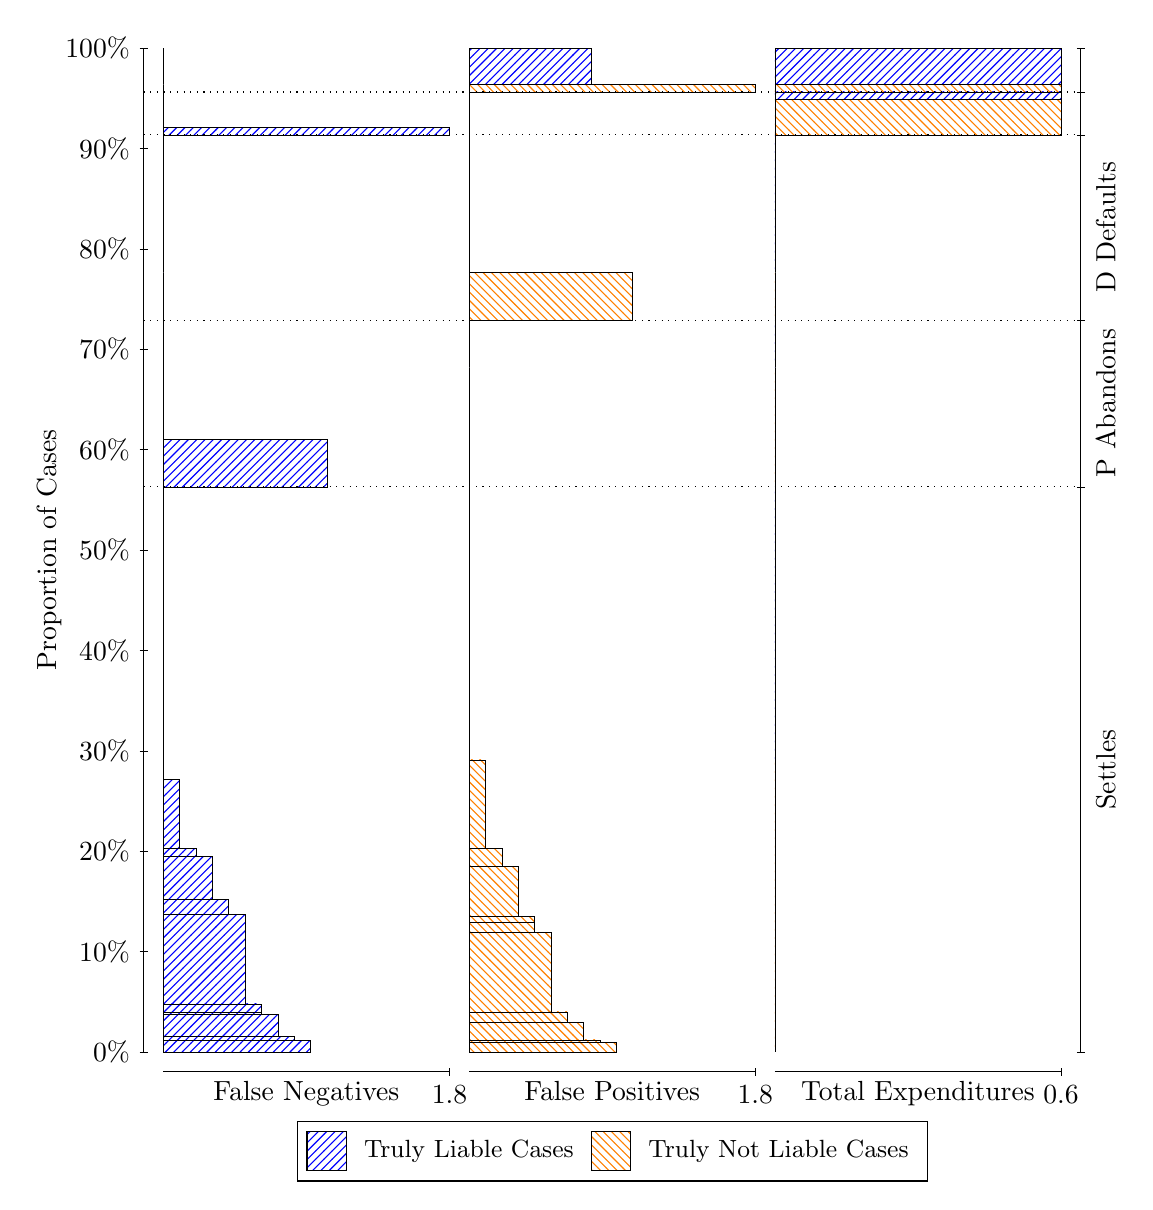
\begin{tikzpicture}
\draw[black, very thin] (1.5,1.75) -- (1.5,14.5);
\node[rotate=90, anchor=center] at (0.3, 8.125) {Proportion of Cases};
\draw[black, very thin] (1.45,1.75) -- (1.55,1.75);
\node[anchor=east] at (1.45, 1.75) {0\%};
\draw[black, very thin] (1.45,3.025) -- (1.55,3.025);
\node[anchor=east] at (1.45, 3.025) {10\%};
\draw[black, very thin] (1.45,4.3) -- (1.55,4.3);
\node[anchor=east] at (1.45, 4.3) {20\%};
\draw[black, very thin] (1.45,5.575) -- (1.55,5.575);
\node[anchor=east] at (1.45, 5.575) {30\%};
\draw[black, very thin] (1.45,6.85) -- (1.55,6.85);
\node[anchor=east] at (1.45, 6.85) {40\%};
\draw[black, very thin] (1.45,8.125) -- (1.55,8.125);
\node[anchor=east] at (1.45, 8.125) {50\%};
\draw[black, very thin] (1.45,9.4) -- (1.55,9.4);
\node[anchor=east] at (1.45, 9.4) {60\%};
\draw[black, very thin] (1.45,10.675) -- (1.55,10.675);
\node[anchor=east] at (1.45, 10.675) {70\%};
\draw[black, very thin] (1.45,11.95) -- (1.55,11.95);
\node[anchor=east] at (1.45, 11.95) {80\%};
\draw[black, very thin] (1.45,13.225) -- (1.55,13.225);
\node[anchor=east] at (1.45, 13.225) {90\%};
\draw[black, very thin] (1.45,14.5) -- (1.55,14.5);
\node[anchor=east] at (1.45, 14.5) {100\%};

\draw[black, very thin] (13.4,1.75) -- (13.4,14.5);
\draw[black, very thin] (13.35,1.75) -- (13.45,1.75);
\node[anchor=west] at (13.35, 1.75) {};
\draw[black, very thin] (13.35,8.927) -- (13.45,8.927);
\node[anchor=west] at (13.35, 8.927) {};
\draw[black, very thin] (13.35,11.044) -- (13.45,11.044);
\node[anchor=west] at (13.35, 11.044) {};
\draw[black, very thin] (13.35,13.398) -- (13.45,13.398);
\node[anchor=west] at (13.35, 13.398) {};
\draw[black, very thin] (13.35,13.942) -- (13.45,13.942);
\node[anchor=west] at (13.35, 13.942) {};
\draw[black, very thin] (13.35,14.5) -- (13.45,14.5);
\node[anchor=west] at (13.35, 14.5) {};

\draw[black, very thin, pattern color=blue, pattern=north east lines] (1.75,1.75) rectangle (3.6186,1.8993);
\draw[black, very thin, pattern color=blue, pattern=north east lines] (1.75,1.8993) rectangle (3.411,1.9501);
\draw[black, very thin, pattern color=blue, pattern=north east lines] (1.75,1.9501) rectangle (3.2033,2.223);
\draw[black, very thin, pattern color=blue, pattern=north east lines] (1.75,2.223) rectangle (2.9957,2.2532);
\draw[black, very thin, pattern color=blue, pattern=north east lines] (1.75,2.2532) rectangle (2.9957,2.3618);
\draw[black, very thin, pattern color=blue, pattern=north east lines] (1.75,2.3618) rectangle (2.7881,3.5015);
\draw[black, very thin, pattern color=blue, pattern=north east lines] (1.75,3.5015) rectangle (2.5805,3.6912);
\draw[black, very thin, pattern color=blue, pattern=north east lines] (1.75,3.6912) rectangle (2.3729,4.2321);
\draw[black, very thin, pattern color=blue, pattern=north east lines] (1.75,4.2321) rectangle (2.1652,4.3387);
\draw[black, very thin, pattern color=blue, pattern=north east lines] (1.75,4.3387) rectangle (1.9576,5.2166);
\draw[black, very thin, pattern color=orange, pattern=north west lines] (1.75,5.2166) rectangle (1.75,8.927);
\draw[black, very thin, pattern color=blue, pattern=north east lines] (1.75,8.927) rectangle (3.8262,9.5284);
\draw[black, very thin, pattern color=orange, pattern=north west lines] (1.75,9.5284) rectangle (1.75,11.044);
\draw[black, very thin, pattern color=orange, pattern=north west lines] (1.75,11.044) rectangle (1.75,11.649);
\draw[black, very thin, pattern color=blue, pattern=north east lines] (1.75,11.649) rectangle (1.75,13.398);
\draw[black, very thin, pattern color=blue, pattern=north east lines] (1.75,13.398) rectangle (5.3833,13.496);
\draw[black, very thin, pattern color=orange, pattern=north west lines] (1.75,13.496) rectangle (1.75,13.942);
\draw[black, very thin, pattern color=orange, pattern=north west lines] (1.75,13.942) rectangle (1.75,14.04);
\draw[black, very thin, pattern color=blue, pattern=north east lines] (1.75,14.04) rectangle (1.75,14.5);
\draw[black, very thin, pattern color=orange, pattern=north west lines] (5.6333,1.75) rectangle (7.5019,1.8732);
\draw[black, very thin, pattern color=orange, pattern=north west lines] (5.6333,1.8732) rectangle (7.2943,1.9022);
\draw[black, very thin, pattern color=orange, pattern=north west lines] (5.6333,1.9022) rectangle (7.0867,2.1292);
\draw[black, very thin, pattern color=orange, pattern=north west lines] (5.6333,2.1292) rectangle (6.879,2.2599);
\draw[black, very thin, pattern color=orange, pattern=north west lines] (5.6333,2.2599) rectangle (6.6714,3.2647);
\draw[black, very thin, pattern color=orange, pattern=north west lines] (5.6333,3.2647) rectangle (6.4638,3.3998);
\draw[black, very thin, pattern color=orange, pattern=north west lines] (5.6333,3.3998) rectangle (6.4638,3.4764);
\draw[black, very thin, pattern color=orange, pattern=north west lines] (5.6333,3.4764) rectangle (6.2562,4.1096);
\draw[black, very thin, pattern color=orange, pattern=north west lines] (5.6333,4.1096) rectangle (6.0486,4.3311);
\draw[black, very thin, pattern color=orange, pattern=north west lines] (5.6333,4.3311) rectangle (5.841,5.4604);
\draw[black, very thin, pattern color=blue, pattern=north east lines] (5.6333,5.4604) rectangle (5.6333,8.927);
\draw[black, very thin, pattern color=orange, pattern=north west lines] (5.6333,8.927) rectangle (5.6333,10.442);
\draw[black, very thin, pattern color=blue, pattern=north east lines] (5.6333,10.442) rectangle (5.6333,11.044);
\draw[black, very thin, pattern color=orange, pattern=north west lines] (5.6333,11.044) rectangle (7.7095,11.649);
\draw[black, very thin, pattern color=blue, pattern=north east lines] (5.6333,11.649) rectangle (5.6333,13.398);
\draw[black, very thin, pattern color=orange, pattern=north west lines] (5.6333,13.398) rectangle (5.6333,13.843);
\draw[black, very thin, pattern color=blue, pattern=north east lines] (5.6333,13.843) rectangle (5.6333,13.942);
\draw[black, very thin, pattern color=orange, pattern=north west lines] (5.6333,13.942) rectangle (9.2667,14.04);
\draw[black, very thin, pattern color=blue, pattern=north east lines] (5.6333,14.04) rectangle (7.1905,14.5);
\draw[black, very thin, pattern color=orange, pattern=north west lines] (9.5167,1.75) rectangle (9.5167,5.4604);
\draw[black, very thin, pattern color=blue, pattern=north east lines] (9.5167,5.4604) rectangle (9.5167,8.927);
\draw[black, very thin, pattern color=orange, pattern=north west lines] (9.5167,8.927) rectangle (9.5167,10.442);
\draw[black, very thin, pattern color=blue, pattern=north east lines] (9.5167,10.442) rectangle (9.5167,11.044);
\draw[black, very thin, pattern color=orange, pattern=north west lines] (9.5167,11.044) rectangle (9.5167,11.649);
\draw[black, very thin, pattern color=blue, pattern=north east lines] (9.5167,11.649) rectangle (9.5167,13.398);
\draw[black, very thin, pattern color=orange, pattern=north west lines] (9.5167,13.398) rectangle (13.15,13.843);
\draw[black, very thin, pattern color=blue, pattern=north east lines] (9.5167,13.843) rectangle (13.15,13.942);
\draw[black, very thin, pattern color=orange, pattern=north west lines] (9.5167,13.942) rectangle (13.15,14.04);
\draw[black, very thin, pattern color=blue, pattern=north east lines] (9.5167,14.04) rectangle (13.15,14.5);
\draw[black, dotted] (1.5,8.927) -- (13.4,8.927);
\draw[black, dotted] (1.5,11.044) -- (13.4,11.044);
\draw[black, dotted] (1.5,13.398) -- (13.4,13.398);
\draw[black, dotted] (1.5,13.942) -- (13.4,13.942);
\draw[black, very thin] (1.75,1.5) -- (5.3833,1.5);
\node[anchor=north] at (3.5667, 1.5) {False Negatives};
\draw[black, very thin] (5.3833,1.45) -- (5.3833,1.55);
\node[anchor=north] at (5.3833, 1.45) {1.8};

\draw[black, very thin] (5.6333,1.5) -- (9.2667,1.5);
\node[anchor=north] at (7.45, 1.5) {False Positives};
\draw[black, very thin] (9.2667,1.45) -- (9.2667,1.55);
\node[anchor=north] at (9.2667, 1.45) {1.8};

\draw[black, very thin] (9.5167,1.5) -- (13.15,1.5);
\node[anchor=north] at (11.333, 1.5) {Total Expenditures};
\draw[black, very thin] (13.15,1.45) -- (13.15,1.55);
\node[anchor=north] at (13.15, 1.45) {0.6};

\node[black, centered, rotate=90] at (13.72, 5.3385) {Settles};
\node[black, centered, rotate=90] at (13.72, 9.9854) {P Abandons};
\node[black, centered, rotate=90] at (13.72, 12.221) {D Defaults};



\draw (7.449999999999999,1.5) node[draw=none] (baseCoordinate) {};
\begin{scope}[align=center]
        \matrix[scale=0.5, draw=black, below=0.5cm of baseCoordinate, nodes={draw}, column sep=0.1cm]{
            \node[rectangle, draw, minimum width=0.5cm, minimum height=0.5cm, pattern=north east lines, pattern color=blue] {}; &
            \node[draw=none, font=\small] (B) {Truly Liable Cases}; &
            \node[rectangle, draw, minimum width=0.5cm, minimum height=0.5cm, pattern=north west lines, pattern color=orange] {}; &
            \node[draw=none, font=\small] (B) {Truly Not Liable Cases}; \\
            };
\end{scope}

\end{tikzpicture}
\end{document}